\documentclass[journal,12pt]{IEEEtran}
\usepackage{cite}      % Written by Donald Arseneau
                        % V1.6 and later of IEEEtran pre-defines the format
                        % of the cite.sty package \cite{} output to follow
                        % that of IEEE. Loading the cite package will
                        % result in citation numbers being automatically
                        % sorted and properly "ranged". i.e.,
                        % [1], [9], [2], [7], [5], [6]
                        % (without using cite.sty)
                        % will become:
                        % [1], [2], [5]--[7], [9] (using cite.sty)
                        % cite.sty's \cite will automatically add leading
                        % space, if needed. Use cite.sty's noadjust option
                        % (cite.sty V3.8 and later) if you want to turn this
                        % off. cite.sty is already installed on most LaTeX
                        % systems. The latest version can be obtained at:
                        % http://www.ctan.org/tex-archive/macros/latex/contrib/supported/cite/

\usepackage{graphicx}  % Written by David Carlisle and Sebastian Rahtz
                        % Required if you want graphics, photos, etc.
                        % graphicx.sty is already installed on most LaTeX
                        % systems. The latest version and documentation can
                        % be obtained at:
                        % http://www.ctan.org/tex-archive/macros/latex/required/graphics/
                        % Another good source of documentation is "Using
                        % Imported Graphics in LaTeX2e" by Keith Reckdahl
                        % which can be found as esplatex.ps and epslatex.pdf
                        % at: http://www.ctan.org/tex-archive/info/

\usepackage{psfrag}    % Written by Craig Barratt, Michael C. Grant,
                        % and David Carlisle
                        % This package allows you to substitute LaTeX
                        % commands for text in imported EPS graphic files.
                        % In this way, LaTeX symbols can be placed into
                        % graphics that have been generated by other
                        % applications. You must use latex->dvips->ps2pdf
                        % workflow (not direct pdf output from pdflatex) if
                        % you wish to use this capability because it works
                        % via some PostScript tricks. Alternatively, the
                        % graphics could be processed as separate files via
                        % psfrag and dvips, then converted to PDF for
                        % inclusion in the main file which uses pdflatex.
                        % Docs are in "The PSfrag System" by Michael C. Grant
                        % and David Carlisle. There is also some information 
                        % about using psfrag in "Using Imported Graphics in
                        % LaTeX2e" by Keith Reckdahl which documents the
                        % graphicx package (see above). The psfrag package
                        % and documentation can be obtained at:
                        % http://www.ctan.org/tex-archive/macros/latex/contrib/supported/psfrag/

\usepackage{subfigure} % Written by Steven Douglas Cochran
                        % This package makes it easy to put subfigures
                        % in your figures. i.e. "figure 1a and 1b"
                        % Docs are in "Using Imported Graphics in LaTeX2e"
                        % by Keith Reckdahl which also documents the graphicx
                        % package (see above). subfigure.sty is already
                        % installed on most LaTeX systems. The latest version
                        % and documentation can be obtained at:
                        % http://www.ctan.org/tex-archive/macros/latex/contrib/supported/subfigure/

\usepackage{url}       % Written by Donald Arseneau
                        % Provides better support for handling and breaking
                        % URLs. url.sty is already installed on most LaTeX
                        % systems. The latest version can be obtained at:
                        % http://www.ctan.org/tex-archive/macros/latex/contrib/other/misc/
                        % Read the url.sty source comments for usage information.

%\usepackage{stfloats}  % Written by Sigitas Tolusis
                        % Gives LaTeX2e the ability to do double column
                        % floats at the bottom of the page as well as the top.
                        % (e.g., "\begin{figure*}[!b]" is not normally
                        % possible in LaTeX2e). This is an invasive package
                        % which rewrites many portions of the LaTeX2e output
                        % routines. It may not work with other packages that
                        % modify the LaTeX2e output routine and/or with other
                        % versions of LaTeX. The latest version and
                        % documentation can be obtained at:
                        % http://www.ctan.org/tex-archive/macros/latex/contrib/supported/sttools/
                        % Documentation is contained in the stfloats.sty
                        % comments as well as in the presfull.pdf file.
                        % Do not use the stfloats baselinefloat ability as
                        % IEEE does not allow \baselineskip to stretch.
                        % Authors submitting work to the IEEE should note
                        % that IEEE rarely uses double column equations and
                        % that authors should try to avoid such use.
                        % Do not be tempted to use the cuted.sty or
                        % midfloat.sty package (by the same author) as IEEE
                        % does not format its papers in such ways.

\usepackage{amsmath}   % From the American Mathematical Society
                        % A popular package that provides many helpful commands
                        % for dealing with mathematics. Note that the AMSmath
                        % package sets \interdisplaylinepenalty to 10000 thus
                        % preventing page breaks from occurring within multiline
                        % equations. Use:
%\interdisplaylinepenalty=2500
                        % after loading amsmath to restore such page breaks
                        % as IEEEtran.cls normally does. amsmath.sty is already
                        % installed on most LaTeX systems. The latest version
                        % and documentation can be obtained at:
                        % http://www.ctan.org/tex-archive/macros/latex/required/amslatex/math/




% *** Do not adjust lengths that control margins, column widths, etc. ***
% *** Do not use packages that alter fonts (such as pslatex).         ***
% There should be no need to do such things with IEEEtran.cls V1.6 and later.


% correct bad hyphenation here
\hyphenation{}


\begin{document}
%
% paper title
\title{The Palladio Component Meta Model:\\ Towards an Engineering Approach\\ to Software Architecture Design}
%
%
% author names and IEEE memberships
% note positions of commas and nonbreaking spaces ( ~ ) LaTeX will not break
% a structure at a ~ so this keeps an author's name from being broken across
% two lines.
% use \thanks{} to gain access to the first footnote area
% a separate \thanks must be used for each paragraph as LaTeX2e's \thanks
% was not built to handle multiple paragraphs
\author{Ralf~Reussner,
        Steffen~Becker,
        and~Jens~Happe% <-this % stops a space
\thanks{Manuscript received January 20, 2002; revised August 13, 2002.}% <-this % stops a space
\thanks{M. Shell is with the Georgia Institute of Technology.}}
% note the % following the last \IEEEmembership and also the first \thanks - 
% these prevent an unwanted space from occurring between the last author name
% and the end of the author line. i.e., if you had this:
% 
% \author{....lastname \thanks{...} \thanks{...} }
%                     ^------------^------------^----Do not want these spaces!
%
% a space would be appended to the last name and could cause every name on that
% line to be shifted left slightly. This is one of those "LaTeX things". For
% instance, "A\textbf{} \textbf{}B" will typeset as "A B" not "AB". If you want
% "AB" then you have to do: "A\textbf{}\textbf{}B"
% \thanks is no different in this regard, so shield the last } of each \thanks
% that ends a line with a % and do not let a space in before the next \thanks.
% Spaces after \IEEEmembership other than the last one are OK (and needed) as
% you are supposed to have spaces between the names. For what it is worth,
% this is a minor point as most people would not even notice if the said evil
% space somehow managed to creep in.
%
% The paper headers
\markboth{IEEE Transactions on Software Engineering,~Vol.~1, No.~8,~August~2002}{Shell}
% The only time the second header will appear is for the odd numbered pages
% after the title page when using the twoside option.


% If you want to put a publisher's ID mark on the page
% (can leave text blank if you just want to see how the
% text height on the first page will be reduced by IEEE)
%\pubid{0000--0000/00\$00.00~\copyright~2002 IEEE}

% use only for invited papers
%\specialpapernotice{(Invited Paper)}

% make the title area
\maketitle


\begin{abstract}
The abstract (100-200 Words).
\end{abstract}

\begin{keywords}
Component, Quality of Service
\end{keywords}


\section{Introduction}
\PARstart{T}{his} is the introduction \cite{balsamo2004b}.
Components are for composition.
Divide and Conquer. 
Provide a hierarchical structure of a software system.
COTS failed. 
But Product-Lines work.

Szyperski's Component:
-	unit of independent deployment
-	unit of third party composition
-	has no (externally) observable state
Our focus: Unit of independent deployment, all agree, but nobody knows what it is. - For us, it is more than copying a DLL.

For the Quality of Service prediction of a software architecture, we need a component model with clear semantics and enough information to conduct analyses. Current component models lack these capabilities.

\section{Components in Software Engineering and Practice}
\label{sec:ComponentsInSE}
What is a software component today?
UML 2.0 (history, UML 1.0 Component = unit of deployment)
-	Encapsulate their contents
-	Are replaceable within its environment
-	Define behaviour in terms of provided and required interfaces

Corba Component Model
J2EE, COM+

SOFA

Software Engineering Processes (RUP, speziell CBSE etc.)

QoS Prediction models (Trivedi, Balsamo, QoSA Reliability Survey Paper)

Cheesman and Daniels

So, what is a Software Component?
o	Realisation
-	Component = class(es) ?
-	How to bind provided and required interfaces?
-	How does the component interact with its environment?
o	Quality of Service
-	Assembly, deployment, internal structure
o	Runtime
-	How does the system look like at runtime?
o	Substitutability and Interoperability

\section{Foundations} % Arbeitstitel!
\label{sec:foundations}

The Palladio component meta modell mainly bases on concepts for
components presented by the OMG in the UML 2.0 standard and parametric contracts
that model the intra-component dependencies of provided and required interfaces.
Both concepts are introduced in the following. 

\subsection{UML 2.0 Component Concepts}

An \emph{assembly connector} connects a required interface of an inner component
to a provided interface
of another inner component. 

\emph{Delegation connectors} map provided and required
interfaces of the composite component to interfaces of its inner
structure. 

A provides delegation connector maps
a provided interface of the composite component to provided interface of an
inner component. 

A requires delegation connector maps a required interface of an
inner component to a required interface of the composite component.


\subsection{Parametric Contracts}

Component contracts lift the Design-by-Contract principle of Meyer (``if a
client fulfils the precondition of a supplier, the supplier guarantees the
postcondition'' \cite{meyer1992a}) from methods to software components. A
component guarantees to offer the functionality specified by its provide
d interfaces (postcondition) if all required interfaces are offered by its
environment. Design-by-Contract cannot only be applied to
functional properties, but also to non-functional properties. Adding Quality of
Service (QoS) attributes to the contract, a component ensures that it
provides a certain QoS if its environment offers the required QoS attributes. 

Parametric contracts \cite{reussner2002c} extend the design by contract
principle of software components. The provided interfaces (postcondition) of a
component are computed in dependence on the actual interfaces offered by the
environment (precondition). The relationship between provided and required
interfaces of a software component can be used to compute the influence of
external services used by the component on its QoS attributes as well. We
distinguish between \emph{basic components} and \emph{composite components} as
two different ways of implementing a component.

We state that a component can still be considered a black-box entity if the
additional information used by parametric contracts (a) does not expose
intellectual property of the component vendor and (b) has not to be understood
by human users. So, the additional information and its analysis has to be
transparent for the deployer.

A \emph{service effect specification} describes the relationship between
provided and required interfaces. It defines the externally visible behaviour of
a provided service. This includes the used external services, possible call
sequences, and, for example, probabilities of service calls. A service effect
specification can be modelled in different ways. It can be a signature list that
only contains the called external services. It can model all possible call
sequences executed by a provided service. This can be expressed by different
means, for example, finite state machines, Petri nets, regular expressions, or
any other kind of grammar. In any case, a service effect specification is an
abstraction of component source code. It models calls to external services only
and neglects the internal component code.

\begin{figure}[htbp]
\centering
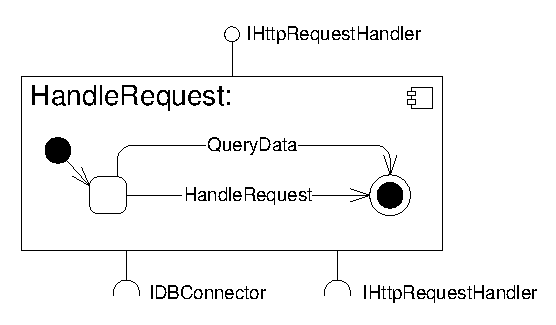
\includegraphics[scale=0.85]{example/HandleRequestSEFF}
\caption{Service effect specification of the method HandleRequest in the
DynamicFileProvider.}
\label{fig:seff}
\end{figure}

Figure \ref{fig:seff} shows a simple service effect specification modelled as a
finite state machine. If the method HandleRequest of the DynamicFileProvider is
responsible for the incoming request it executes a query on the connected
database. In the internal code that is not visible here, it creates the web page
and returns the result to the client. If it is not responsible for the incoming
request it forwards the request to the next component in the chain of
responsibility. This is done by the call of the HandleRequest method of the
component connected to the IHttpRequestHandler interface.



%
% $Id$
%
% $Log$
% Revision 1.4  2005/10/26 14:44:10  sbecker
% Restructured
% Focus on:
% - Subtyping
% - Valid Signatures
% - Protocols
%
%

\section{Interfaces} %Steffen

In the book by Szyperski et al. the section on components and interfaces starts with

\begin{quote}
"`Interfaces are the means by which components connect \cite[p. 50]{szyperski2002a}."'
\end{quote}

For components interfaces are a key concept as they serve multiple purposes. As in object oriented languages, which have the concept of interfaces, they can be used to build a type system as introduced in section \ref{types_design_by_contract}. In our model interfaces can have an arbitrary amount of super-interfaces. A common constraint for the hierarchy of interfaces is that any given interface can not be supertype of itself, which gives us a acyclic subtype hierarchy.

In order to define a subtype relationship on interfaces, consider an interface taken from common programming languages like Java or C\#. There, an interface specifies a set of operation signatures, consisting of an operation name, its parameter names and type, return types and exceptions. In our model we have some constraints on the types which can be used. As the external view of components is characterized by its interfaces, only interface references and basic data types (integer, string, ...) are allowed but no component references.

Interfaces are applied to specify the allowed communication between communicating entities. The contracts specified in the interface (method contracts, invariants) characterize the valid behaviour of these entities. In object oriented languages an object can act in two roles with respect to an interface: server or client. In the server role, the object "`implements"' or "`realizes"' the operations specified in the interfaces and observes the method pre- and postconditions. In the client role, the object calls services offered in a given interface by fulfilling the precondition and expecting the postcondition. However, in both cases the interface and its associated contracts serve both roles as contract on which they can rely.
 
As with legal contracts, interfaces can exist even when no one actually declared their commitment to them, i.e., there is no specific client or server. For example, this is used to define a certain set of standardised interfaces of a library to enable the construction of clients and servers of these libraries independently. Thus, in the Palladio Component Meta Model the concept \emph{Interface} exists as first class entity which can be specified independent from other entities.

% TODO: + JMS Beispiel

The specification of the contract which is represented by an interface can be enhanced by including a specification of the sequence in which the interface's operations can be used. This kind of information is called a protocol. The protocol is a special class of the more general concept of arbitrary preconditions for methods. Any kind of protocol can be expressed via preconditions. Thus, the protocol is an abstraction of the set of all preconditions. The abstraction is often made based on the expressiveness of the used specification formalism. For example, consider using finite state machines as protocol specification formalism. With this formalism it is impossible to express the valid call sequences of a stack exactly (the amount of push calls always has to be equal or greater then the amount of pop calls). Nevertheless, FSM-protocols can be analysed with quite efficient algorithms. 

Using the information described above, the subtype relationship of any two arbitrary interfaces $I_1,I_2$ can be specified as follows. Interface $I_1$ is subtype of $I_2$ if it is able to fulfil at least the contracts of $I_2$. In detail, this means it has to be able to handle all the (single) method calls which $I_2$ can handle. Additionally, it must also at least support the call sequences which $I_2$ supports.

% Hence, the analysis of the subtype relationship is essential for modelling a component based architecture and is therefore part of our component model. The information available can be further used to allow semi- and fully automatic adaptation of components, e.g., by using the Adapter design pattern \cite{gamma1995a}.

However, having the concept of signatures and their protocol, there a still some open questions. For example, Szyperski et al. \cite{szyperski2002a} highlight some subtle problems in component communication resulting from additional concepts which are also important during the interaction of components. The insufficient specification of multi-threaded interaction, re-entrance or transactional behaviour are only examples of ongoing research in this field. Additionally, there are no widely established formalisms to specify Quality of Service constraints on a contractual basis. Hence, as there are no settled results in these fields of research yet, our model currently only includes the concepts of signatures and basic protocol information.
%
% $Id$
%
% $Log$
% Revision 1.2  2005/10/26 14:35:52  sbecker
% Started section on provided interfaces
%
%

\section{Interface Relations}

An interface protocol is used to characterise a set of allowed call sequences sent by a client to a server. However the actual meaning of the protocol of the interface depends on its relationship to a specific component. TODO: Soll das wirklich hier hin? Provided und Required Roles/Ports?
\section{Component Types}
With the introduction of software components, the question of their substitutability and conformance arises. A component is not only defined by its provided interfaces, but also by the interfaces required from the environment. So, the constraints for replacing a component in its context are more complex than, for example, the constraints for replacing a class that implements a set of interfaces. The UML 2.0 superstructure addresses this issue only curtly:

\begin{quote}
``As such, a component serves as a type whose conformance is defined by these provided and required interfaces $[\ldots]$. One component may therefore be substituted by another only if the two are type conformant \cite[p.142]{OMGUML2005a}.''
%TODO add reference: UML Superstructure p.150
\end{quote}

Here, the terms \emph{component type} and \emph{conformance} of components and types are mentioned. However, both concepts are not further clarified. We need a clear definition of both terms to provide a component meta model that allows (a)  interoperability and substitutability checks of components and (b) enables the prediction of Quality of Service attributes of a component in a certain context.

In the following, we develop a more detailed approach to component types that allows different notions of substitutability. We also clarify the conformance of a component to a type. We introduce these concepts using the architecture of a web server shown in figure \ref{fig:WebserverComponents} and give a formal definition of the terms at the end of this section.

\begin{figure}[htbp]
\centering
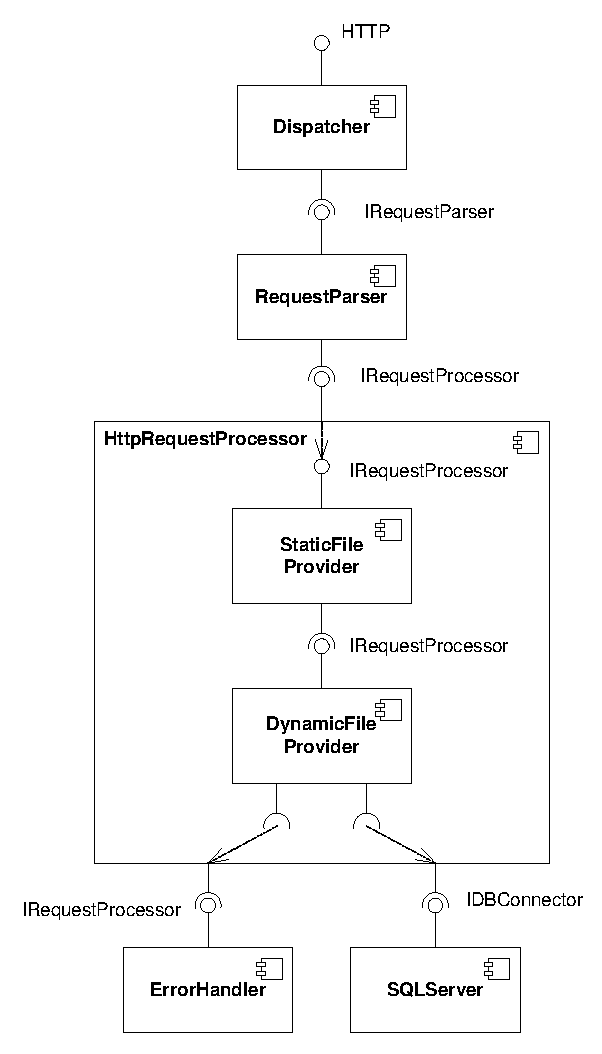
\includegraphics[width=3.3in]{example/WebserverComponents}
\caption{Component architecture of a web server.}
\label{fig:WebserverComponents}
\end{figure}

The main part of the web server is realised by the three components Dispatcher, RequestParser, and HttpRequestProcessor. The Dispatcher listens on a set of incoming connections. For each incoming HTTP request, it spawns a new tread and activates the RequestParser. The parser analyses the request and passes the result to the HttpRequestProcessor. The request processor is organised as a chain of responsability \cite{gamma1995a}. Each of its subcomponents checks whether it can handle the incoming request. If so, it returns the result, otherwise it passes the request to the next component in the chain of responsibility. The ErrorHandler represents the end of the chain and returns an error message if the request could not be handled by any of the components. Additionally, the SQLServer is required to create dynamic HTML pages.


\begin{figure}[htbp]
\centering
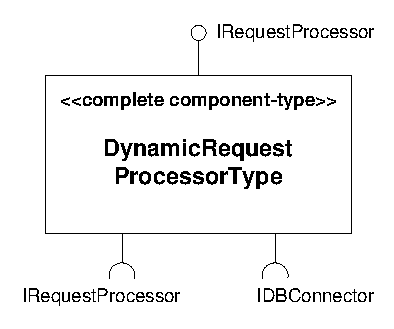
\includegraphics[scale=0.85]{example/DynamicRequestProcessorType}
\caption{Component type for dynamic request processors.}
\label{fig:DynamicRequestProcessorType}
\end{figure}

Looking at the architecture of the web server, we can identify different component types according to the definition in UML 2.0. For example, the components HttpRequestProcessor and DynamicFileProvide provide the IRequestProcessor interface and use the interfaces IDBConnector and IRequestProcessor. The first one is used to create dynamic content of web pages. The second one is required to forward the request to the next component in the chain of responsibility. The corresponding type of both components is shown in figure \ref{fig:DynamicRequestProcessorType}.

\begin{figure}[htbp]
\centering
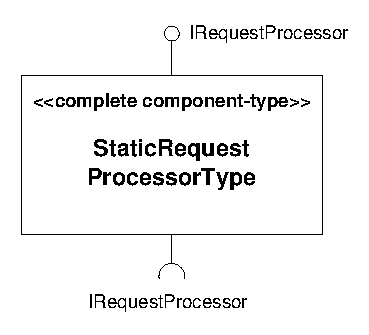
\includegraphics[scale=0.85]{example/RequestProcessorType}
\caption{Another component type used in the web server.}
\label{fig:RequestProcessorType}
\end{figure}

The type of the StaticFileProvider component shown in figure \ref{fig:RequestProcessorType} provides and requires the IRequestProcessor interface only. So, it differs from the DynamicRequestProcessorType, which additionally requires the IDBConnector interface. 

The types shown in figures \ref{fig:DynamicRequestProcessorType} and \ref{fig:RequestProcessorType} are derived from existing components and describe their complete provided and required functionality.
It is obvious that a component conforms to a type if it provides and requires exactly the interfaces specified by the type. However, this is not the case in general. A component is likely to differ from its more general type, but, nevertheless, still be conformant to the type. So, when does a component conform to a type?

A component conforms to a type, if it offers at least the functionality specified by the provided interfaces of the type and uses only the functionality specified by the required interfaces of the type.

For example, a component must offer the IRequestProcessor interface to conform to one of the types in figure \ref{fig:DynamicRequestProcessorType} or \ref{fig:RequestProcessorType}, but it can provide additional interfaces.
Furthermore, a component can only use services that are specified in the required interfaces of the type. The DynamicFileProvider does not conform to the RequestProcessorType, since it uses the IDBConnector interface. Note that a component does not have to use all required interfaces of its type. So, all components that conform to the RequestProcessorType also conform to the DynamicRequestProcessorType, since they do not require the IDBConnectorInterface. 

The definition of conformance corresponds to our view on required and provided interfaces as pre- and postcondition of components (see section \ref{sec:ComponentImplementation}). The precondition can only be strengthened. Thus, the component implementation must not use interfaces other than the required interfaces specified by the type. Furthermore, the postcondition can only be weakened. The component can offer any interfaces, but it must at least provide the ones specified by the type. With this notion of conformance, the type system of components is contravariant.

This understanding of conformance between components and types allows us to define substitutability of components. A component \texttt{A} can be substituted by a component \texttt{B} if \texttt{B} conforms to the type defined by \texttt{A}. The type defined by a component includes all its provided and required interfaces. This is a very pessimistic definition of substitutability, which can be weakened under certain conditions. 

In many cases, we are not only interested in the substitution of complete components including provided and required interfaces, but in a substitution with respect to provided interfaces only. This is the case if the functionality is more important than the requirements of a component or if we compare the functionality offered by different components. 

\begin{figure}[htbp]
\centering
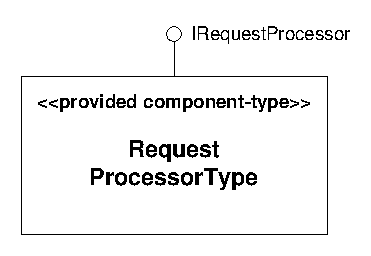
\includegraphics[scale=0.85]{example/ProvidesType}
\caption{Provides-type of the RequestProcessorType and DynamicRequestProcessorType.}
\label{fig:ProvidesType}
\end{figure}

Hence, we want to allow conformance with respect to provided interfaces only. Therefore, we introduce a \emph{provides-type} which only contains provided interfaces. The provides-type of the RequestProcessortType and the DynamicRequestProcessorType is shown in figure \ref{fig:ProvidesType}. 


This is not the only Type that is used in the component model of the web server.

So, some components provide the same interfaces, but require different services to complete their task.
Distinguish between Provided and Complete types. Both have their advantages. They are defined by substitutability. 

The development process of a component is not fixed to both types of a component, but is an evolutionary process.
During Software architecture design, there is no clear border between both types.

The stepwise completion of a component specification leads to different interpretations of required interfaces.
-	can be used, but there can be more (provided type interpretation)
-	can only be used (complete type)
-	has to be used in a predefined fashion (not considered in our case, example: information has to be stored in a database, so the interface of the database must be used.

Conformance between Provided and Complete Types.

%\section{Component Implementation Description}
\label{sec:ComponentImplementation}

In general, a component model does not provide any information about the inner structure of its components, since components are regarded as a black box entities. However, black-box components inhibit the analysis of Quality of Service (QoS) attributes of the system, since important information about the dependency of these attributes on external services, hardware and software resources, and the usage profile cannot be specified. Static QoS contracts, like the QoS Modelling Language (QML) \cite{frolund1998a}, are also not sufficient for this task. If the required QoS profile of a component cannot be provided by the environment, the component is likely to work, but with lower quality. 

Therefore, we need additional information on the inner component structure to analyse the QoS attributes of software components at design time.

Provided and required interfaces as pre and postcondition

Basic Component
Service effect specification

Composite Component
Assembly/Delegation Connector 
Today: theoretical construct no physical representation.

Conforms Relation to the Complete Type

Description of the inner component structure. Type? -  In theory there might be different implementation that conform to the same description as in MDA. But since in most cases, this is a one to one relationship. We don't care.

-- Overview --

Benefit: Parametric Contracts (Example)

\section{Deployment}
The step of placing or installing software on the target systems. This includes configuration steps if necessary.

General understanding for software components: Placement of a component in an execution environment.

Our understanding:
The deployment of a software component defines its context.
1.	Assembling of components (Connections)
2.	Allocation of components on resources

Both steps can be done independently (two roles, different persons). Nowadays they are generally considered as deployment.

A component can be embedded into different contexts, since it is a unit of independent deployment. This can happen several times within the same system. Leaving type theory.

Within the same system, we have that the same component has different contexts, including the wiring, the mapping to resources and the containment.

Explicit modelling of the context. 
Two dimensions: Assembly and Allocation, Computed vs. Specified Values.

--Table with different context aspects--

Assembly and allocation can contain special configurations of a component.

Connections and their deployment: Today, either fixed connection between components or naming services. Both do not allow individual connection of components. So, components are no real units of independent deployment at the moment. Technical realisation required.

Composite Components can only be deployed as one piece.
Resource diagram and assembly diagram are specified independently. 

Communication nodes, which only model network structures.

\section{Deployment of Connections}
Deployment of Connections on paths (a path describes the route between two nodes, acyclic)

-- Overview --

\section{Components at Runtime}
Cardinalities

Concurrency modelling

Benefit: QoS Prediction
\section{Conclusion}
Future Work
-	MOF-Schema and OCL-Constraints
-	MDA-Transforms
-	Description approximating the run-time view of the system (virtual interactors)
-	Modelling of concurrency, asynchronous method calls
-	QoS analysis
-	Process model for CBSE with the Palladio Component Meta Model


\section*{Acknowledgments}
Thanks to everyone.

\bibliography{palladio}
\bibliographystyle{plain}

% The very first letter is a 2 line initial drop letter followed
% by the rest of the first word in caps.
% 
% form to use if the first word consists of a single letter:
% \PARstart{A}{demo} file is ....
% 
% form to use if you need the single drop letter followed by
% normal text (unknown if ever used by IEEE):
% \PARstart{A}{}demo file is ....
% 
% Some journals put the first two words in caps:
% \PARstart{T}{his demo} file is ....
% 
% Here we have the typical use of a "T" for an initial drop letter
% and "HIS" in caps to complete the first word.
% \PARstart{T}{his} demo file is intended to serve as a ``starter file"
% for IEEE journal papers produced under \LaTeX\ using IEEEtran.cls version
% 1.6 and later.
% You must have at least 2 lines in the paragraph with the drop letter
% (should never be an issue)
% May all your publication endeavors be successful.

%\hfill mds

%\hfill August 13, 2002

%\subsection{Subsection Heading Here}
%Subsection text here.

% needed in second column of first page if using \pubid
%\pubidadjcol

%\subsubsection{Subsubsection Heading Here}
%Subsubsection text here.

% Reminder: the "draftcls", not "draft", class option should be used if
% it is desired that the figures are to be displayed while in draft mode.

% An example of a floating figure using the graphicx package.
% Note that \label must occur AFTER (or within) \caption.
% For figures, \caption should occur after the \includegraphics.
%
%\begin{figure}
%\centering
%\includegraphics[width=2.5in]{myfigure.eps}
%\caption{Simulation Results}
%\label{fig_sim}
%\end{figure}


% An example of a double column floating figure using two subfigures.
% (The subfigure.sty package must be loaded for this to work.)
% The subfigure \label commands are set within each subfigure command, the
% \label for the overall fgure must come after \caption.
% \hfil must be used as a separator to get equal spacing
%
%\begin{figure*}
%\centerline{\subfigure[Case I]{\includegraphics[width=2.5in]{subfigcase1.eps}
%\label{fig_first_case}}
%\hfil
%\subfigure[Case II]{\includegraphics[width=2.5in]{subfigcase2.eps}
%\label{fig_second_case}}}
%\caption{Simulation results}
%\label{fig_sim}
%\end{figure*}



% An example of a floating table. Note that, for IEEE style tables, the 
% \caption command should come BEFORE the table. Table text will default to
% \footnotesize as IEEE normally uses this smaller font for tables.
% The \label must come after \caption as always.
%
%\begin{table}
%% increase table row spacing, adjust to taste
%\renewcommand{\arraystretch}{1.3}
%\caption{An Example of a Table}
%\label{table_example}
%\centering
%% The array package and the MDW tools package offers better commands
%% for making tables than plain LaTeX2e's tabular which is used here.
%\begin{tabular}{|c||c|}
%\hline
%One & Two\\
%\hline
%Three & Four\\
%\hline
%\end{tabular}
%\end{table}


%\section{Conclusion}
%The conclusion goes here.

% if have a single appendix:
%\appendix[Proof of the Zonklar Equations]
% or
%\appendix  % for no appendix heading
% do not use \section anymore after \appendix, only \section*
% is possibly needed

% use appendices with more than one appendix
% then use \section to start each appendix
% you must declare a \section before using any
% \subsection or using \label (\appendices by itself
% starts a section numbered zero.)
%
% Use this command to get the appendices' numbers in "A", "B" instead of the
% default capitalized Roman numerals ("I", "II", etc.).
% However, the capital letter form may result in awkward subsection numbers
% (such as "A-A"). Capitalized Roman numerals are the default.
%\useRomanappendicesfalse
%
%\appendices
%\section{Proof of the First Zonklar Equation}
%Appendix one text goes here.

% you can choose not to have a title for an appendix
% if you want by leaving the argument blank
%\section{}
%Appendix two text goes here.

% use section* for acknowledgement
%\section*{Acknowledgment}
% optional entry into table of contents (if used)
%\addcontentsline{toc}{section}{Acknowledgment}
%The authors would like to thank... This work was supported by the IEEE.

% trigger a \newpage just before the given reference
% number - used to balance the columns on the last page
% adjust value as needed - may need to be readjusted if
% the document is modified later
%\IEEEtriggeratref{8}
% The "triggered" command can be changed if desired:
%\IEEEtriggercmd{\enlargethispage{-5in}}

% references section
% NOTE: BibTeX documentation can be easily obtained at:
% http://www.ctan.org/tex-archive/biblio/bibtex/contrib/doc/

% can use a bibliography generated by BibTeX as a .bbl file
% standard IEEE bibliography style from:
% http://www.ctan.org/tex-archive/macros/latex/contrib/supported/IEEEtran/
%\bibliographystyle{IEEEtran.bst}
% argument is your BibTeX string definitions and bibliography database(s)
%\bibliography{IEEEabrv,../bib/paper}
%
% <OR> manually copy in the resultant .bbl file
% set second argument of \begin to the number of references
% (used to reserve space for the reference number labels box)

%\begin{thebibliography}{1}

%\bibitem{IEEEhowto:kopka}
%This is an example of a book reference
%H. Kopka and P.W. Daly, \emph{A Guide to {\LaTeX}}, third ed. Harlow, U.K.: Addison-Wesley, 1999.

%This is an example of a article reference
%A. Gefen, ``Simulations of Foot Stability During Gait Characteristic of Ankle Dorsiflexor Weakness
%in the Elderly,'' \emph{IEEE Trans. Neural Systems Rehabilitation Eng.,} vol. 9, no. 4, pp. 333-337, Dec. 2001.

%This is an example of a article from a conference proceeding
%T. Tuytelaars and L. van Gool ``Content-Based Image Retrieval Based on Local Affinely Invariant Regions,''
%\emph{Proc. Third Int'l Conf. Visual Information Systems,} pp. 493-500, 1999.

%Again, see the IEEEtrans_HOWTO.pdf for several more bibliographical examples. Also, more style examples 
%can be seen at http://www.computer.org/author/style/transref.htm 

%\end{thebibliography}

% biography section
% 
% If you had an eps/pdf photo file (graphicx package needed)
% the extra braces prevent the LaTeX parser from getting confused
% when it sees the complicated \includegraphics command within an
% optional argument. You can create your own macro to make things
% simpler here.
%\begin{biography}[{\includegraphics[width=1in,height=1.25in,clip,keepaspectratio]{mshell.eps}}]{Michael Shell}
% or if you just want to reserve a space for a photo:

%\begin{biography}{Michael Shell}
%Biography text here.
%\end{biography}

% if you will not have a photo
%\begin{biographynophoto}{John Doe}
%Biography text here.
%\end{biographynophoto}

% insert where needed to balance the two columns on the last page
%\newpage

%\begin{biographynophoto}{Jane Doe}
%Biography text here.
%\end{biographynophoto}

% You can push biographies down or up by placing
% a \vfill before or after them. The appropriate
% use of \vfill depends on what kind of text is
% on the last page and whether or not the columns
% are being equalized.

%\vfill

% Can be used to pull up biographies so that the bottom of the last one
% is flush with the other column.
%\enlargethispage{-5in}

% that's all folks
\end{document}


